\clearpage
\section*{Appendix B. Laboratory, source and proposer sensitivity}
\label{app:core}
\setcounter{table}{0}
\renewcommand{\thetable}{B.\arabic{table}}
\renewcommand{\theHtable}{B.\arabic{table}}
\paragraph{Completed study design.}
This appendix reports completed follow-up evaluations with the same target scorers as the main study. Laboratory-count experiments cover all five endpoints at $K\in\{1,2,5,10\}$ under both increasing participation and a fixed total data pool. DTI uses seed 61; the lighter proteomics and cell experiments use seeds 61--63. Independent-source DTI and proteomics use seed 61, and external-source VCC uses seeds 61--63. The two-proposer study has two separate protocols: a 12-design, six-slot study on all five endpoints (DTI seed 42; other endpoints seed 61), and a 36-design, 24-slot study on the four lighter endpoints at seed 61. Each candidate receives 100 training rounds. The latter changes the design space as well as the search budget, so budget comparisons are made within a protocol. Main-table results retain their original seeds 42--44 and protocol.

\subsection*{B.1 Number of laboratories}
The participation experiment uses a fixed nested set of the first $K$ original clients, increasing both training and development access. The fixed-pool experiment merges the complete ten-client pool into $K$ training groups while retaining equal-weight evaluation over the original ten development panels. Thus its selection population stays fixed as training partitions change. The identical $K=10$ fit is reused by both comparisons. Every unique fit uses the default design and 100 rounds. The cell objective forms contrastive negatives within each local training group, so repartitioning changes the negative pool as well as optimization steps. These comparisons characterize the implemented training pipeline at different collaboration scales. Zero between-seed SD can occur when a fixed pretrained head receives an identical single-batch update; it describes training variability on these fixed partitions.

\begin{table}[htbp]
\centering\small
\setlength{\tabcolsep}{4pt}
\begin{tabularx}{\linewidth}{@{}lXrrrr@{}}
\toprule
Task & Metric & $K=1$ & $K=2$ & $K=5$ & $K=10$ \\
\midrule
DTI & AUROC & 83.65 & 84.43 & 89.62 & \textbf{93.88} \\
PTPC & AP & 26.03 $\pm$ 5.57 & 37.38 $\pm$ 0.60 & 29.63 $\pm$ 2.50 & \textbf{37.54 $\pm$ 0.27} \\
VCC & Macro Top-1 & 30.02 $\pm$ 0.78 & \textbf{39.56 $\pm$ 0.11} & 31.88 $\pm$ 0.00 & 31.48 $\pm$ 0.16 \\
Norman & Macro Top-1 & \textbf{25.56 $\pm$ 0.00} & 18.22 $\pm$ 0.00 & 19.68 $\pm$ 1.11 & 15.48 $\pm$ 0.00 \\
Tahoe & Macro Top-1 & 19.40 $\pm$ 0.00 & 25.37 $\pm$ 0.00 & 20.90 $\pm$ 0.00 & \textbf{26.37 $\pm$ 0.86} \\
\bottomrule
\end{tabularx}
\caption{Increasing participation. A nested set of the original ten client partitions participates, so increasing $K$ also adds training data. The default design and 100-round trainer are fixed. DTI uses seed 61; the four light endpoints report mean $\pm$ sample SD over seeds 61--63. Scores are metric $\times100$; bold denotes the best $K$ within each row, including displayed ties.}
\label{tab:completed-participation}
\end{table}

\begin{table}[htbp]
\caption{Fixed data pool. All target data are retained and merged into $K$ clients; only the partition count changes. The default design and 100-round trainer are fixed. DTI uses seed 61; the four light endpoints report mean $\pm$ sample SD over seeds 61--63. Scores are metric $\times100$; bold denotes the best $K$ within each row, including displayed ties.}
\label{tab:completed-partition}
\centering\small
\setlength{\tabcolsep}{4pt}
\begin{tabularx}{\linewidth}{@{}lXrrrr@{}}
\toprule
Task & Metric & $K=1$ & $K=2$ & $K=5$ & $K=10$ \\
\midrule
DTI & AUROC & 85.47 & 88.96 & 88.05 & \textbf{93.88} \\
PTPC & AP & 34.59 $\pm$ 5.66 & 37.36 $\pm$ 1.89 & \textbf{39.19 $\pm$ 0.43} & 37.54 $\pm$ 0.27 \\
VCC & Macro Top-1 & 29.49 $\pm$ 0.00 & 28.80 $\pm$ 0.20 & 31.06 $\pm$ 0.22 & \textbf{31.48 $\pm$ 0.16} \\
Norman & Macro Top-1 & \textbf{49.63 $\pm$ 4.20} & 19.56 $\pm$ 0.20 & 26.12 $\pm$ 0.11 & 15.48 $\pm$ 0.00 \\
Tahoe & Macro Top-1 & 22.39 $\pm$ 0.00 & 21.39 $\pm$ 0.86 & 20.40 $\pm$ 0.86 & \textbf{26.37 $\pm$ 0.86} \\
\bottomrule
\end{tabularx}
\end{table}


\subsection*{B.2 Independent sources and target evaluation}
For DTI and cell transfer, the entire target training pool is one study-level client. Each auxiliary collection contributes a separate local update through sample-weighted aggregation. Only the original target development panels select the checkpoint; every configuration is evaluated on the same target test set. Target-only, individual-source and combined-source configurations start from the same task initialization.

DTI auxiliaries are BioSNAP, Davis and Human from the pinned TAPB release, with 19,092, 1,721 and 2,929 retained training pairs after drug--protein-pair de-duplication against target splits and preceding sources. All five DTI source configurations complete the same 100-round schedule. VCC auxiliary data comprise Replogle K562, Nadig HepG2 and Jiang IFNB/K562, with respectively 60, 60 and 58 retained training interventions \citep{replogle2022perturbseq,nadig2025trade,jiang2025pathways}. Source feature panels preserve measured genes, and target development/test intervention identities are excluded from source training. The source manifest records retained subsets, feature intersections and exclusions.

\begin{table}[htbp]
\centering\small
\setlength{\tabcolsep}{4pt}
\begin{tabularx}{\linewidth}{@{}lXlrr@{}}
\toprule
Target & Additional source & Metric & Score $\uparrow$ & $\Delta$ (pp) \\
\midrule
DTI & Target only & AUROC & 85.47 & +0.00 \\
DTI & + BioSNAP & AUROC & 82.44 & -3.03 \\
DTI & + Davis & AUROC & 87.86 & +2.39 \\
DTI & + Human & AUROC & \textbf{87.95} & +2.48 \\
DTI & + All three & AUROC & 84.30 & -1.18 \\
\midrule
VCC & Target only & Macro Top-1 & 29.49 $\pm$ 0.00 & +0.00 $\pm$ 0.00 \\
VCC & + Replogle & Macro Top-1 & 27.12 $\pm$ 0.08 & -2.37 $\pm$ 0.08 \\
VCC & + Nadig & Macro Top-1 & 26.94 $\pm$ 0.18 & -2.55 $\pm$ 0.18 \\
VCC & + Jiang & Macro Top-1 & \textbf{33.07 $\pm$ 0.00} & +3.58 $\pm$ 0.00 \\
VCC & + All three & Macro Top-1 & 27.33 $\pm$ 0.00 & -2.15 $\pm$ 0.00 \\
\midrule
PTPC auxiliary & Target only & AP & 34.98 & +0.00 \\
PTPC auxiliary & + Lin & AP & 35.01 & +0.03 \\
PTPC auxiliary & + Ruprecht & AP & \textbf{35.50} & +0.52 \\
PTPC auxiliary & + Both & AP & 35.31 & +0.34 \\
\bottomrule
\end{tabularx}
\caption{Independent-source transfer on the same target heldout set, including every prespecified source and their combination. DTI (seed 61) adds BioSNAP, Davis or Human; VCC (seeds 61--63, mean $\pm$ SD) adds Replogle, Nadig or Jiang. The PTPC auxiliary multi-task model (seed 61) adds Lin or Ruprecht and is compared only with its matched auxiliary target-only model. PTPC has two independent external studies, not three. Changes are paired against target-only training; bold marks the best score within a target/model block. Scores are multiplied by 100.}
\label{tab:completed-independent-transfer}
\end{table}


The cell study reports mean and SD across three seeds together with a paired intervention-bootstrap analysis. Jiang improves target Top-1 by 3.58 points; its 95\% bootstrap interval is [$-$2.11, 9.51]. This positive point estimate motivates further source-aware evaluation, while the complete table also exposes sources whose updates reduce the target metric.

\paragraph{Independent proteomics pilot.}
Two independent lung-cancer studies provide auxiliary measurements: Lin et al.\ \citep{Lin2026HDAC} and Ruprecht et al.\ \citep{Ruprecht2020Proteome}. Their continuous response labels differ from the binary target endpoint. A shared masked-protein encoder of width 64 and drug encoder of width 32 therefore feed source-specific prediction heads. Target fitting uses its binary efficacy objective; Lin predicts continuous CellTiter-Glo response, and Ruprecht predicts an interval-valued potency outcome. Target data retain the original ten clients; Lin and Ruprecht each add one study-level client. Shared encoders use sample-weighted aggregation, whereas each private head is updated only by its own source clients. The common local-worker and coordinator interfaces are reused. This adapter is compared against its own target-only control, separately from the main-table PTPC predictor.

The Lin subset contains 28 drug conditions (20 source-training, eight source-development), spanning five training and two development drugs. Inputs are 24-hour, 10-$\mu$M protein log-fold changes, and the response is the mean of the three released CellTiter-Glo ratio measurements. The HCT16/HCT116 alias is excluded from auxiliary training. The Ruprecht subset contains 109 matched drug conditions (85 training, 24 development; 17 and five drugs respectively). Protein log-fold changes at 24 hours are paired with CellTiter-Glo EC50 values in $\log_{10}$ nM: 49 exact, 18 approximate and 42 right-censored outcomes. Squared distance to the encoded potency interval is the loss. The adapter treats explicit lower bounds and values at or above 10,000 nM as right-censored and encodes approximate values with a factor-of-two interval; these are analysis conventions. Profiling dose is not a model input; source acquisition nevertheless uses dose conditions chosen in relation to drug response. The target retains 386 training and 105 development examples, with 148 held-out observations across 92 compounds and 22 positives.

All four source settings receive the same 100-round procedure. A two-proposal Luna loop is also executed independently for each setting. These 12 fits and eight valid proposal calls produce eight fixed/loop evaluations. Fixed and loop selection have identical held-out ranking scores in each source arm (Table~\ref{tab:completed-protein-loop}). The source effect and the proposal-history effect are thus measured separately.

\begin{table}[htbp]
\caption{Independent-source proteomics auxiliary pilot, seed 61. Fixed design and a two-proposal Luna loop use the same shared-encoder/source-specific-head model and 100-round training allocation. Every source arm and both selection modes are retained. The heldout AP gain from this short loop is zero in all four source conditions; source-transfer gains are a different comparison.}
\label{tab:completed-protein-loop}
\centering\small
\setlength{\tabcolsep}{4pt}
\begin{tabularx}{\linewidth}{@{}Xlrr@{}}
\toprule
Training sources & Selection & AP $\uparrow$ & $\Delta$ vs target only (pp) \\
\midrule
Target only & Fixed & 34.98 & +0.00 \\
Target only & Loop & 34.98 & +0.00 \\
+ Lin & Fixed & 35.01 & +0.03 \\
+ Lin & Loop & 35.01 & +0.03 \\
+ Ruprecht & Fixed & \textbf{35.50} & +0.52 \\
+ Ruprecht & Loop & \textbf{35.50} & +0.52 \\
+ Both & Fixed & 35.31 & +0.34 \\
+ Both & Loop & 35.31 & +0.34 \\
\bottomrule
\end{tabularx}
\end{table}


Target-only AP/AUROC are 34.98/74.75. Adding Lin yields 35.01/74.78, Ruprecht 35.50/74.28 and both 35.31/74.17. Paired compound bootstrap (1,000 resamples) gives 95\% intervals for the AP changes of [$-$0.20, 0.28], [$-$1.46, 2.64] and [$-$1.62, 2.49] points, respectively. These results measure transfer from two independent external studies. The three cell-line contexts below answer a separate, within-study question.

\paragraph{Within-study proteomic contexts.}
HCC1143, HCC1806 and MDA-MB-453-1 are drawn from the mtPTDS supplementary collection \citep{Sun2026ProteinTalks}, each with 47 retained drug conditions and 3,501 proteins shared with the target panel. They are three biological contexts within one study. Target development/test compounds are excluded from source training. These experiments use the original proteomic adapter and seeds 61--63.

\begin{table}[htbp]
\centering\small
\setlength{\tabcolsep}{4pt}
\begin{tabularx}{\linewidth}{@{}Xrrr@{}}
\toprule
Additional context & AP $\uparrow$ & $\Delta$ AP (pp) & Paired 95\% CI \\
\midrule
Target only & 34.59 $\pm$ 5.66 & +0.00 $\pm$ 0.00 & [0.00, 0.00] \\
+ HCC1143 & 34.94 $\pm$ 5.15 & +0.35 $\pm$ 0.56 & [-1.22, 1.60] \\
+ HCC1806 & 35.23 $\pm$ 5.35 & +0.64 $\pm$ 0.32 & [-0.78, 1.77] \\
+ MDA-MB-453-1 & 35.20 $\pm$ 5.31 & +0.61 $\pm$ 0.44 & [-0.85, 2.04] \\
+ All three & \textbf{35.47 $\pm$ 6.36} & +0.87 $\pm$ 8.89 & [-2.44, 3.99] \\
\bottomrule
\end{tabularx}
\caption{Within-study PTPC context transfer, reported separately from independent-source transfer. HCC1143, HCC1806 and MDA-MB-453-1 belong to the same mtPTDS study. Values are mean $\pm$ sample SD over seeds 61--63, multiplied by 100. Confidence intervals resample target compounds while retaining paired seed predictions. These contexts are not additional independent studies; the original model and results are unchanged.}
\label{tab:completed-context-transfer}
\end{table}


\clearpage
\subsection*{B.3 Research-model and six-slot proposal comparison}
The short study uses the 12 executable designs of Appendix A. Direct search receives untried identifiers without measured scores; the loop additionally receives accumulated development evidence. Both modes share initialization and the first proposal. Each slot allows two attempts to return the four-field proposal schema; failed slots consume budget and remain in the trace. Every valid candidate restarts from the common task/seed initialization and is fitted for 100 rounds. Prefixes at 0, 1, 2, 4 and 6 slots are evaluated after the trajectory is complete. An exact fit cache can reuse an identical configuration while retaining its logical training-budget charge.

Qwen uses the local sampling settings in Appendix A. The second proposer is the \texttt{gpt-5.6-luna} service, accessed in a text-only session with tool use disabled; request metadata and responses are retained. The comparison holds task messages, editable designs, training procedure and proposal budget fixed across backends. Service-level decoding controls and parameter count are not exposed by the Luna interface.

\begin{table}[htbp]
\centering\small
\setlength{\tabcolsep}{4pt}
\begin{tabularx}{\linewidth}{@{}Xlrrr@{}}
\toprule
Task & Proposer & Fixed & Direct@6 & Loop@6 \\
\midrule
DTI & Luna & 94.27 & \textbf{94.60} & 94.27 \\
DTI & Qwen & \textbf{94.27} & \textbf{94.27} & \textbf{94.27} \\
PTPC & Luna & \textbf{37.27} & \textbf{37.27} & \textbf{37.27} \\
PTPC & Qwen & \textbf{37.27} & \textbf{37.27} & \textbf{37.27} \\
VCC & Luna & \textbf{31.50} & \textbf{31.50} & \textbf{31.50} \\
VCC & Qwen & \textbf{31.50} & \textbf{31.50} & \textbf{31.50} \\
Norman & Luna & 15.48 & 22.30 & \textbf{23.11} \\
Norman & Qwen & 15.48 & \textbf{22.30} & \textbf{22.30} \\
Tahoe & Luna & 25.37 & \textbf{26.87} & \textbf{26.87} \\
Tahoe & Qwen & \textbf{25.37} & \textbf{25.37} & \textbf{25.37} \\
\bottomrule
\end{tabularx}
\caption{Original 12-design/six-slot heldout results. DTI seed 42; four light endpoints seed 61. All displayed budgets are prefixes of this single protocol; they are not selected by test performance. Every candidate uses 100 rounds. Scores use each original task metric $\times100$; bold marks the best displayed score within a row, including ties.}
\label{tab:completed-short6}
\end{table}

\begin{table}[htbp]
\caption{Original 12-design/six-slot search dynamics. DTI seed 42; four light endpoints seed 61. D/L means direct/loop. The common target is the lower of the two terminal development primary scores, so it is attainable by both runs; first records its earliest attainment. Last gain is the last strictly improving primary-score slot; last retain also includes loss-tiebreak selections. These are retrospective diagnostics, not stopping rules. Slot 0 is initialization.}
\label{tab:completed-dynamics-short6}
\centering\small
\setlength{\tabcolsep}{4pt}
\begin{tabularx}{\linewidth}{@{}Xlrrrrr@{}}
\toprule
Task & Proposer & Dev. target & First D/L & Last gain D/L & Last retain D/L & Valid D/L \\
\midrule
DTI & Luna & 94.71 & 0/0 & 6/0 & 6/0 & 6/6 \\
DTI & Qwen & 94.71 & 0/0 & 0/0 & 0/0 & 6/6 \\
PTPC & Luna & 66.72 & 0/0 & 0/0 & 0/0 & 6/6 \\
PTPC & Qwen & 66.72 & 0/0 & 0/0 & 0/0 & 6/5 \\
VCC & Luna & 24.04 & 3/6 & 3/6 & 3/6 & 6/6 \\
VCC & Qwen & 23.65 & 0/0 & 0/0 & 0/0 & 6/6 \\
Norman & Luna & 51.70 & 5/5 & 5/5 & 5/5 & 6/6 \\
Norman & Qwen & 51.70 & 3/4 & 3/4 & 3/4 & 6/6 \\
Tahoe & Luna & 30.00 & 0/0 & 0/0 & 6/3 & 6/6 \\
Tahoe & Qwen & 30.00 & 0/0 & 0/0 & 0/0 & 4/4 \\
\bottomrule
\end{tabularx}
\end{table}


All five endpoints have both backends and both search modes. Among the ten direct/loop pairs, Norman/Luna improves by 0.81 Top-1 points, DTI/Luna decreases by 0.33 AUROC points and eight pairs tie. The twenty DTI prefix scores were independently recomputed from saved predictions for all 5,505 test pairs, with checkpoint and output hashes verified. The curves below show the complete prespecified prefix sequence for every endpoint, alongside its development selection trajectory.

\begin{figure}[htbp]
\centering
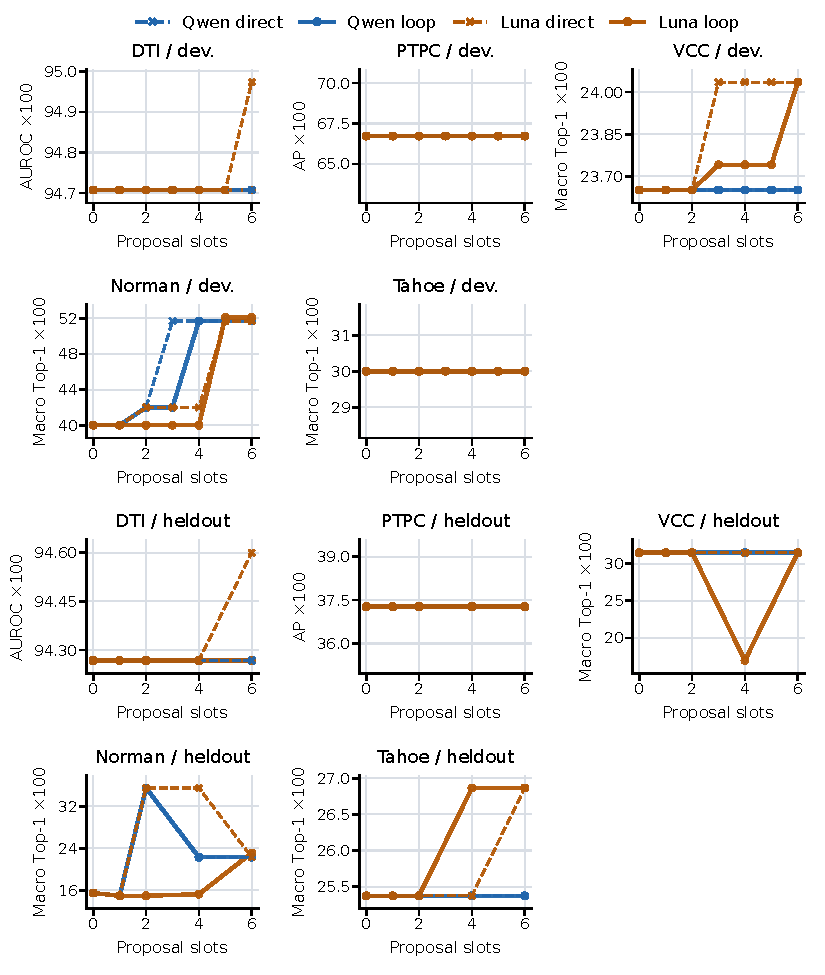
\includegraphics[width=\linewidth]{assets/completed_short6_search.pdf}
\caption{Development selection (upper panels) and held-out performance (lower panels) in the 12-design, six-slot protocol across all five endpoints. Each valid proposal receives the same full fitting schedule; failed slots still consume research budget. Slot 0 is initialization. Held-out curves evaluate the development-selected checkpoints at every prespecified prefix.}
\label{fig:completed-short-dev}
\end{figure}

\clearpage
\subsection*{B.4 Extended search and task-dependent saturation}
The extended study increases the design library to 36 configurations: three learning rates, three weight decays, two server-momentum values and two residual-head settings. It runs 24 proposal slots for both backends and modes on PTPC, VCC, Norman and Tahoe. Prefixes are 0, 1, 2, 4, 6, 8, 12, 16, 20 and 24. The settings for initialization, full candidate fitting, development selection and invalid-slot accounting are otherwise unchanged. DTI's backend comparison is the completed six-slot study in B.3; it is not part of this extended protocol.

\begin{table}[htbp]
\centering\small
\setlength{\tabcolsep}{4pt}
\begin{tabularx}{\linewidth}{@{}Xlrrrrr@{}}
\toprule
Task & Proposer & Fixed & Direct@6 & Loop@6 & Direct@24 & Loop@24 \\
\midrule
PTPC & Luna & \textbf{37.27} & \textbf{37.27} & \textbf{37.27} & \textbf{37.27} & \textbf{37.27} \\
PTPC & Qwen & \textbf{37.27} & \textbf{37.27} & \textbf{37.27} & \textbf{37.27} & \textbf{37.27} \\
VCC & Luna & \textbf{31.50} & 16.94 & 16.94 & 20.23 & 20.01 \\
VCC & Qwen & \textbf{31.50} & \textbf{31.50} & \textbf{31.50} & 19.61 & 19.61 \\
Norman & Luna & 15.48 & \textbf{35.48} & 23.11 & 23.11 & 23.11 \\
Norman & Qwen & 15.48 & \textbf{22.30} & \textbf{22.30} & \textbf{22.30} & \textbf{22.30} \\
Tahoe & Luna & 25.37 & 13.43 & \textbf{26.87} & 13.43 & 13.43 \\
Tahoe & Qwen & 25.37 & \textbf{26.87} & \textbf{26.87} & 13.43 & 13.43 \\
\bottomrule
\end{tabularx}
\caption{Extended 36-design/24-slot heldout results. Four light endpoints, seed 61; no native DTI 24-slot result is implied. All displayed budgets are prefixes of this single protocol; they are not selected by test performance. Every candidate uses 100 rounds. Scores use each original task metric $\times100$; bold marks the best displayed score within a row, including ties.}
\label{tab:completed-long24}
\end{table}

\begin{table}[htbp]
\centering\small
\setlength{\tabcolsep}{4pt}
\begin{tabularx}{\linewidth}{@{}Xlrrrrr@{}}
\toprule
Task & Proposer & Dev. target & First D/L & Last gain D/L & Last retain D/L & Valid D/L \\
\midrule
PTPC & Luna & 66.72 & 0/0 & 0/0 & 0/0 & 24/24 \\
PTPC & Qwen & 66.72 & 0/0 & 0/0 & 0/0 & 19/14 \\
VCC & Luna & 27.68 & 16/9 & 16/10 & 16/10 & 24/24 \\
VCC & Qwen & 24.83 & 18/23 & 18/23 & 18/23 & 11/16 \\
Norman & Luna & 52.10 & 22/4 & 22/4 & 22/7 & 24/24 \\
Norman & Qwen & 51.70 & 2/5 & 2/5 & 22/19 & 15/12 \\
Tahoe & Luna & 35.00 & 5/13 & 5/13 & 5/13 & 24/24 \\
Tahoe & Qwen & 35.00 & 18/14 & 18/14 & 18/14 & 14/15 \\
\bottomrule
\end{tabularx}
\caption{Extended 36-design/24-slot search dynamics. Four light endpoints, seed 61; no native DTI 24-slot result is implied. D/L means direct/loop. The common target is the lower of the two terminal development primary scores, so it is attainable by both runs; first records its earliest attainment. Last gain is the last strictly improving primary-score slot; last retain also includes loss-tiebreak selections. These are retrospective diagnostics, not stopping rules. Slot 0 is initialization.}
\label{tab:completed-dynamics-long24}
\end{table}


Luna produces valid designs in all 192 attempted slots, and Qwen in 116 of 192. Across 16 mode trajectories, the primary development score is unchanged in the final eight slots in 12 cases; the full score/loss selection key is unchanged in ten. Each trajectory retains 11--24 unvisited designs. A plateau therefore characterizes finite-budget search with a particular backend, rather than exhaustion of the design space.

Table~\ref{tab:completed-dynamics-long24} measures the first slot attaining the smaller terminal development score within each direct/loop pair, a common target reached by both modes. Luna reaches Norman's common target earlier with feedback (4 versus 22 slots), whereas direct search reaches Tahoe's target earlier (5 versus 13). Proteomics retains the initial design. Table~\ref{tab:completed-norman-events} connects Norman's trajectory to concrete configuration changes: reducing the learning rate to $10^{-4}$ gives an early development gain, and removing the residual head reaches the final primary-score target. Subsequent loss-tiebreak selections can change the retained design without increasing that primary score.


The eight terminal held-out pairs give seven ties and one decrease with feedback (VCC/Luna, $-0.22$ points). Within this extended protocol, Qwen's VCC held-out Top-1 decreases from 31.50 at slot 6 to 19.61 at slot 24 while development selection improves. This separates the speed of finding a strong development design from generalization of the selected predictor. The complete development and held-out curves support task-specific budget analysis alongside the proposal-validity and remaining-space diagnostics.

\begin{figure}[htbp]
\centering
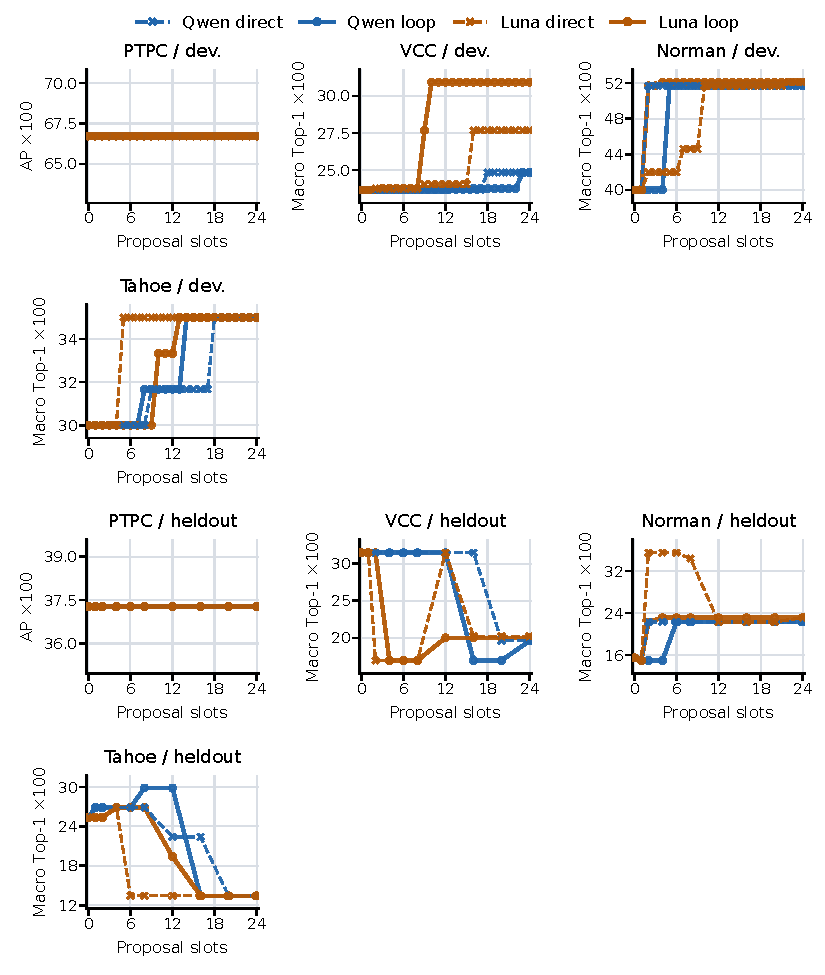
\includegraphics[width=\linewidth]{assets/completed_long24_search.pdf}
\caption{Development selection (upper panels) and held-out performance (lower panels) in the separate 36-design, 24-slot protocol on four endpoints. Curves are paired within the same backend, initialization and design space. Score plateaus may still include loss-tiebreak selections. All prespecified prefixes are displayed. Six-slot points here belong to this 36-design protocol, not the separate 12-design experiment.}
\label{fig:completed-long-dev}
\end{figure}

\clearpage
\subsection*{B.5 Executed designs and proposal traces}
Tables~\ref{tab:completed-menu-short6} and \ref{tab:completed-menu-long24} decode the two design libraries. Tables~\ref{tab:completed-trace-short6} and \ref{tab:completed-trace-long24} retain all 504 attempted proposal slots and their acceptance decisions: 120 slots in the short protocol and 384 in the extended protocol. The accompanying machine-readable trace additionally records each proposal's full configuration, changes from the incumbent and measured development score. Together with the prefix curves, these records connect research decisions to both the executable intervention and its observed outcome.

\begin{table}[htbp]
\caption{All retained proposals for the Norman/Luna extended 36-design, 24-slot study, seed 61. The two modes share initialization and first proposal. lr, wd, m and R denote learning rate, weight decay, server momentum and residual-head indicator. Development selection is followed by evaluation at every prespecified heldout prefix; the full attempted-slot trace is retained separately.}
\label{tab:completed-norman-events}
\centering\small
\setlength{\tabcolsep}{4pt}
\begin{tabularx}{\linewidth}{@{}llXr@{}}
\toprule
Mode & Slot & Executed configuration & Dev. Top-1 \\
\midrule
Direct & 0 & Common initial recipe & 40.00 \\
Direct & 1 & lr=0.001, wd=0.001, m=0, R=1 & 40.00 \\
Direct & 2 & lr=0.001, wd=0.001, m=0.9, R=1 & 42.00 \\
Direct & 7 & lr=0.001, wd=0.01, m=0.9, R=1 & 44.60 \\
Direct & 10 & lr=0.0001, wd=0, m=0, R=1 & 51.70 \\
Direct & 11 & lr=0.0001, wd=0.001, m=0, R=1 & 51.70 \\
Direct & 22 & lr=0.0001, wd=0.001, m=0, R=0 & 52.10 \\
Loop & 0 & Common initial recipe & 40.00 \\
Loop & 1 & lr=0.001, wd=0.001, m=0, R=1 & 40.00 \\
Loop & 2 & lr=0.0001, wd=0.001, m=0, R=1 & 51.70 \\
Loop & 4 & lr=0.0001, wd=0.001, m=0, R=0 & 52.10 \\
Loop & 7 & lr=0.0001, wd=0, m=0, R=0 & 52.10 \\
\bottomrule
\end{tabularx}
\end{table}

\begin{table}[htbp]
\caption{Twelve executable configurations for the short6 protocol. Every design has proximal coefficient zero. A trace design ID uniquely identifies these parameter changes; the task-specific prediction interface remains fixed.}
\label{tab:completed-menu-short6}
\centering\small
\setlength{\tabcolsep}{4pt}
\begin{tabularx}{\linewidth}{@{}Xrrrr@{}}
\toprule
Design & Learning rate & Weight decay & Server momentum & Residual head \\
\midrule
D00 & 0.001 & 0.001 & 0 & No \\
D01 & 0.0001 & 0.001 & 0 & No \\
D02 & 0.01 & 0.001 & 0 & No \\
D03 & 0.001 & 0 & 0 & No \\
D04 & 0.001 & 0.01 & 0 & No \\
D05 & 0.001 & 0.001 & 0.9 & No \\
D06 & 0.001 & 0.001 & 0 & Yes \\
D07 & 0.001 & 0.001 & 0.9 & Yes \\
D08 & 0.0001 & 0.001 & 0 & Yes \\
D09 & 0.0001 & 0.001 & 0.9 & Yes \\
D10 & 0.01 & 0.01 & 0 & No \\
D11 & 0.001 & 0.01 & 0 & Yes \\
\bottomrule
\end{tabularx}
\end{table}

\begin{table}[htbp]
\centering\small
\setlength{\tabcolsep}{4pt}
\begin{tabularx}{\linewidth}{@{}Xrrrr@{}}
\toprule
Design & Learning rate & Weight decay & Server momentum & Residual head \\
\midrule
L0W0M0R0 & 0.0001 & 0 & 0 & No \\
L0W0M0R1 & 0.0001 & 0 & 0 & Yes \\
L0W0M1R0 & 0.0001 & 0 & 0.9 & No \\
L0W0M1R1 & 0.0001 & 0 & 0.9 & Yes \\
L0W1M0R0 & 0.0001 & 0.001 & 0 & No \\
L0W1M0R1 & 0.0001 & 0.001 & 0 & Yes \\
L0W1M1R0 & 0.0001 & 0.001 & 0.9 & No \\
L0W1M1R1 & 0.0001 & 0.001 & 0.9 & Yes \\
L0W2M0R0 & 0.0001 & 0.01 & 0 & No \\
L0W2M0R1 & 0.0001 & 0.01 & 0 & Yes \\
L0W2M1R0 & 0.0001 & 0.01 & 0.9 & No \\
L0W2M1R1 & 0.0001 & 0.01 & 0.9 & Yes \\
L1W0M0R0 & 0.001 & 0 & 0 & No \\
L1W0M0R1 & 0.001 & 0 & 0 & Yes \\
L1W0M1R0 & 0.001 & 0 & 0.9 & No \\
L1W0M1R1 & 0.001 & 0 & 0.9 & Yes \\
L1W1M0R0 & 0.001 & 0.001 & 0 & No \\
L1W1M0R1 & 0.001 & 0.001 & 0 & Yes \\
L1W1M1R0 & 0.001 & 0.001 & 0.9 & No \\
L1W1M1R1 & 0.001 & 0.001 & 0.9 & Yes \\
L1W2M0R0 & 0.001 & 0.01 & 0 & No \\
L1W2M0R1 & 0.001 & 0.01 & 0 & Yes \\
L1W2M1R0 & 0.001 & 0.01 & 0.9 & No \\
L1W2M1R1 & 0.001 & 0.01 & 0.9 & Yes \\
L2W0M0R0 & 0.01 & 0 & 0 & No \\
L2W0M0R1 & 0.01 & 0 & 0 & Yes \\
L2W0M1R0 & 0.01 & 0 & 0.9 & No \\
L2W0M1R1 & 0.01 & 0 & 0.9 & Yes \\
L2W1M0R0 & 0.01 & 0.001 & 0 & No \\
L2W1M0R1 & 0.01 & 0.001 & 0 & Yes \\
L2W1M1R0 & 0.01 & 0.001 & 0.9 & No \\
L2W1M1R1 & 0.01 & 0.001 & 0.9 & Yes \\
L2W2M0R0 & 0.01 & 0.01 & 0 & No \\
L2W2M0R1 & 0.01 & 0.01 & 0 & Yes \\
L2W2M1R0 & 0.01 & 0.01 & 0.9 & No \\
L2W2M1R1 & 0.01 & 0.01 & 0.9 & Yes \\
\bottomrule
\end{tabularx}
\caption{Thirty-six executable configurations for the long24 protocol. Every design has proximal coefficient zero. A trace design ID uniquely identifies these parameter changes; the task-specific prediction interface remains fixed.}
\label{tab:completed-menu-long24}
\end{table}

\clearpage
\begingroup\small
\setlength{\tabcolsep}{3pt}
\begin{longtable}{@{}p{0.10\linewidth}p{0.08\linewidth}p{0.08\linewidth}>{\raggedright\arraybackslash}p{0.66\linewidth}@{}}
\caption{Complete proposal trace for short6. Each token is slot:design:decision, with A=retained, R=not retained, I=invalid. Design configurations are decoded in Table~\ref{tab:completed-menu-short6}. All proposed slots, including failures, are retained. Full configuration deltas and development scores are in the accompanying snapshot and TSV.}\label{tab:completed-trace-short6}\\
\toprule Task & Proposer & Mode & Slot:design:decision \\ \midrule\endfirsthead
\toprule Task & Proposer & Mode & Slot:design:decision \\ \midrule\endhead
\bottomrule\endfoot
DTI & Luna & Direct & 1:D06:R; 2:D05:R; 3:D04:R; 4:D07:R; 5:D03:R; 6:D11:A \\[3pt]
DTI & Luna & Loop & 1:D06:R; 2:D08:R; 3:D05:R; 4:D04:R; 5:D03:R; 6:D01:R \\[3pt]
DTI & Qwen & Direct & 1:D06:R; 2:D07:R; 3:D08:R; 4:D09:R; 5:D04:R; 6:D05:R \\[3pt]
DTI & Qwen & Loop & 1:D06:R; 2:D07:R; 3:D08:R; 4:D09:R; 5:D04:R; 6:D05:R \\[3pt]
PTPC & Luna & Direct & 1:D06:R; 2:D05:R; 3:D03:R; 4:D07:R; 5:D04:R; 6:D11:R \\[3pt]
PTPC & Luna & Loop & 1:D06:R; 2:D08:R; 3:D05:R; 4:D04:R; 5:D11:R; 6:D03:R \\[3pt]
PTPC & Qwen & Direct & 1:D06:R; 2:D07:R; 3:D08:R; 4:D09:R; 5:D04:R; 6:D05:R \\[3pt]
PTPC & Qwen & Loop & 1:D06:R; 2:D10:R; 3:D07:R; 4:D08:R; 5:--:I; 6:D09:R \\[3pt]
VCC & Luna & Direct & 1:D06:R; 2:D07:R; 3:D03:A; 4:D04:R; 5:D05:R; 6:D11:R \\[3pt]
VCC & Luna & Loop & 1:D06:R; 2:D04:R; 3:D05:A; 4:D09:R; 5:D02:R; 6:D03:A \\[3pt]
VCC & Qwen & Direct & 1:D06:R; 2:D07:R; 3:D08:R; 4:D09:R; 5:D04:R; 6:D11:R \\[3pt]
VCC & Qwen & Loop & 1:D06:R; 2:D07:R; 3:D10:R; 4:D08:R; 5:D04:R; 6:D09:R \\[3pt]
Norman & Luna & Direct & 1:D06:A; 2:D07:A; 3:D05:R; 4:D03:R; 5:D08:A; 6:D11:R \\[3pt]
Norman & Luna & Loop & 1:D06:A; 2:D11:R; 3:D05:R; 4:D04:A; 5:D01:A; 6:D09:R \\[3pt]
Norman & Qwen & Direct & 1:D06:A; 2:D07:A; 3:D08:A; 4:D09:R; 5:D04:R; 6:D11:R \\[3pt]
Norman & Qwen & Loop & 1:D06:A; 2:D07:A; 3:D11:R; 4:D08:A; 5:D10:R; 6:D05:R \\[3pt]
Tahoe & Luna & Direct & 1:D06:R; 2:D03:R; 3:D05:R; 4:D07:R; 5:D08:R; 6:D11:A \\[3pt]
Tahoe & Luna & Loop & 1:D06:R; 2:D05:R; 3:D04:A; 4:D11:R; 5:D10:R; 6:D03:R \\[3pt]
Tahoe & Qwen & Direct & 1:--:I; 2:D06:R; 3:D07:R; 4:--:I; 5:D08:R; 6:D09:R \\[3pt]
Tahoe & Qwen & Loop & 1:--:I; 2:D06:R; 3:--:I; 4:D07:R; 5:D09:R; 6:D05:R \\[3pt]
\end{longtable}
\endgroup

\begingroup\small
\setlength{\tabcolsep}{3pt}
\begin{longtable}{@{}p{0.10\linewidth}p{0.08\linewidth}p{0.08\linewidth}>{\raggedright\arraybackslash}p{0.66\linewidth}@{}}
\caption{Complete proposal trace for long24. Each token is slot:design:decision, with A=retained, R=not retained, I=invalid. Design configurations are decoded in Table~\ref{tab:completed-menu-long24}. All proposed slots, including failures, are retained. Full configuration deltas and development scores are in the accompanying snapshot and TSV.}\label{tab:completed-trace-long24}\\
\toprule Task & Proposer & Mode & Slot:design:decision \\ \midrule\endfirsthead
\toprule Task & Proposer & Mode & Slot:design:decision \\ \midrule\endhead
\bottomrule\endfoot
PTPC & Luna & Direct & 1:L1W1M1R1:R; 2:L1W1M0R1:R; 3:L1W1M1R0:R; 4:L1W2M1R1:R; 5:L0W1M0R1:R; 6:L1W2M0R0:R; 7:L2W1M0R0:R; 8:L1W0M0R1:R; 9:L1W0M1R0:R; 10:L1W2M0R1:R; 11:L1W0M0R0:R; 12:L1W2M1R0:R; 13:L0W1M1R1:R; 14:L0W1M0R0:R; 15:L1W0M1R1:R; 16:L0W1M1R0:R; 17:L2W1M0R1:R; 18:L0W2M0R0:R; 19:L0W2M0R1:R; 20:L2W1M1R0:R; 21:L2W2M0R1:R; 22:L0W2M1R1:R; 23:L0W0M1R0:R; 24:L0W0M0R1:R \\[3pt]
PTPC & Luna & Loop & 1:L1W1M1R1:R; 2:L1W2M0R0:R; 3:L1W1M0R1:R; 4:L0W1M0R0:R; 5:L1W1M1R0:R; 6:L1W2M0R1:R; 7:L0W0M0R1:R; 8:L1W0M0R1:R; 9:L0W1M0R1:R; 10:L2W1M0R0:R; 11:L2W2M0R1:R; 12:L2W2M0R0:R; 13:L0W1M1R0:R; 14:L0W0M1R0:R; 15:L1W2M1R0:R; 16:L0W1M1R1:R; 17:L1W2M1R1:R; 18:L0W2M1R0:R; 19:L2W1M0R1:R; 20:L0W2M0R0:R; 21:L0W0M0R0:R; 22:L0W2M0R1:R; 23:L2W0M1R1:R; 24:L0W0M1R1:R \\[3pt]
PTPC & Qwen & Direct & 1:L1W0M0R1:R; 2:L0W0M0R1:R; 3:L1W0M1R1:R; 4:L1W1M1R1:R; 5:L1W2M1R1:R; 6:L0W0M1R1:R; 7:L1W1M0R1:R; 8:L0W1M0R1:R; 9:L0W1M1R1:R; 10:L2W2M1R1:R; 11:L2W0M1R1:R; 12:--:I; 13:L1W2M1R0:R; 14:L2W2M0R1:R; 15:--:I; 16:L2W1M1R1:R; 17:--:I; 18:L2W1M0R1:R; 19:--:I; 20:L1W1M1R0:R; 21:--:I; 22:L2W0M0R1:R; 23:L2W2M1R0:R; 24:L0W2M0R1:R \\[3pt]
PTPC & Qwen & Loop & 1:L1W0M0R1:R; 2:L1W0M0R0:R; 3:--:I; 4:L0W0M0R1:R; 5:L0W0M1R1:R; 6:L0W1M1R1:R; 7:--:I; 8:L0W1M0R1:R; 9:L1W1M1R1:R; 10:--:I; 11:--:I; 12:L1W0M1R1:R; 13:L1W1M0R1:R; 14:L2W2M1R1:R; 15:L1W2M1R1:R; 16:--:I; 17:--:I; 18:--:I; 19:L0W2M0R1:R; 20:L1W1M1R0:R; 21:--:I; 22:L1W2M0R1:R; 23:--:I; 24:--:I \\[3pt]
VCC & Luna & Direct & 1:L1W1M0R1:R; 2:L1W1M1R0:A; 3:L1W1M1R1:R; 4:L1W2M0R1:R; 5:L1W2M1R1:R; 6:L1W0M0R1:R; 7:L1W2M1R0:R; 8:L1W2M0R0:R; 9:L1W0M0R0:A; 10:L0W1M0R1:R; 11:L2W1M0R0:R; 12:L1W0M1R0:R; 13:L1W0M1R1:R; 14:L2W1M1R1:R; 15:L2W1M0R1:R; 16:L2W1M1R0:A; 17:L0W1M0R0:R; 18:L0W1M1R1:R; 19:L0W1M1R0:R; 20:L2W2M0R1:R; 21:L0W2M0R1:R; 22:L0W0M0R1:R; 23:L2W0M0R0:R; 24:L0W2M1R1:R \\[3pt]
VCC & Luna & Loop & 1:L1W1M0R1:R; 2:L2W2M0R0:R; 3:L1W1M1R0:A; 4:L0W1M1R0:R; 5:L1W1M1R1:R; 6:L1W0M1R0:R; 7:L1W2M1R0:R; 8:L0W0M1R1:R; 9:L2W1M1R0:A; 10:L2W2M1R0:A; 11:L2W2M1R1:R; 12:L1W2M1R1:R; 13:L1W2M0R0:R; 14:L1W0M0R0:R; 15:L1W0M1R1:R; 16:L2W2M0R1:R; 17:L1W2M0R1:R; 18:L0W1M0R0:R; 19:L1W0M0R1:R; 20:L2W1M0R0:R; 21:L2W1M0R1:R; 22:L0W1M0R1:R; 23:L2W1M1R1:R; 24:L0W0M0R0:R \\[3pt]
VCC & Qwen & Direct & 1:L1W1M1R1:R; 2:L1W1M0R1:R; 3:L0W0M0R1:R; 4:L0W0M1R1:R; 5:--:I; 6:--:I; 7:L0W1M0R1:R; 8:L1W2M1R1:R; 9:--:I; 10:--:I; 11:--:I; 12:L0W1M1R0:R; 13:--:I; 14:--:I; 15:--:I; 16:--:I; 17:--:I; 18:L2W2M1R1:A; 19:L1W0M1R1:R; 20:--:I; 21:--:I; 22:--:I; 23:L0W1M1R1:R; 24:L1W2M0R1:R \\[3pt]
VCC & Qwen & Loop & 1:L1W1M1R1:R; 2:L0W0M1R1:R; 3:L1W0M0R1:R; 4:--:I; 5:L0W0M0R1:R; 6:--:I; 7:L0W1M1R1:R; 8:L0W1M0R1:R; 9:L1W1M0R1:R; 10:L1W2M1R1:R; 11:L1W2M1R0:R; 12:L0W2M0R1:R; 13:L1W1M1R0:A; 14:--:I; 15:L1W0M1R1:R; 16:--:I; 17:--:I; 18:L2W0M1R1:R; 19:--:I; 20:L1W2M0R1:R; 21:--:I; 22:L2W1M1R1:R; 23:L2W2M1R1:A; 24:--:I \\[3pt]
Norman & Luna & Direct & 1:L1W1M0R1:A; 2:L1W1M1R1:A; 3:L1W0M0R1:R; 4:L1W1M1R0:R; 5:L1W0M1R0:R; 6:L1W2M0R1:R; 7:L1W2M1R1:A; 8:L1W2M0R0:R; 9:L1W0M1R1:R; 10:L0W0M0R1:A; 11:L0W1M0R1:A; 12:L1W2M1R0:R; 13:L0W1M1R1:R; 14:L2W1M0R1:R; 15:L1W0M0R0:R; 16:L2W1M0R0:R; 17:L2W1M1R1:R; 18:L2W2M1R1:R; 19:L2W0M0R1:R; 20:L2W2M0R1:R; 21:L2W0M1R1:R; 22:L0W1M0R0:A; 23:L2W1M1R0:R; 24:L0W1M1R0:R \\[3pt]
Norman & Luna & Loop & 1:L1W1M0R1:A; 2:L0W1M0R1:A; 3:L0W1M1R1:R; 4:L0W1M0R0:A; 5:L0W1M1R0:R; 6:L0W2M0R0:R; 7:L0W0M0R0:A; 8:L0W2M0R1:R; 9:L1W0M0R0:R; 10:L0W0M0R1:R; 11:L1W0M0R1:R; 12:L0W0M1R0:R; 13:L1W1M1R0:R; 14:L1W2M0R0:R; 15:L0W2M1R0:R; 16:L0W2M1R1:R; 17:L0W0M1R1:R; 18:L2W1M0R0:R; 19:L1W1M1R1:R; 20:L1W2M0R1:R; 21:L1W2M1R0:R; 22:L2W2M0R0:R; 23:L1W0M1R0:R; 24:L1W0M1R1:R \\[3pt]
Norman & Qwen & Direct & 1:L1W1M0R1:A; 2:L0W0M0R1:A; 3:L0W1M1R1:R; 4:--:I; 5:L1W1M1R1:R; 6:L0W0M1R1:R; 7:--:I; 8:L2W2M1R1:R; 9:L0W1M0R1:A; 10:--:I; 11:L1W2M0R1:R; 12:L1W2M1R1:R; 13:--:I; 14:--:I; 15:--:I; 16:--:I; 17:L2W2M0R1:R; 18:L2W1M0R1:R; 19:L2W0M1R1:R; 20:L2W1M1R1:R; 21:--:I; 22:L0W2M0R1:A; 23:--:I; 24:L1W0M0R1:R \\[3pt]
Norman & Qwen & Loop & 1:L1W1M0R1:A; 2:--:I; 3:--:I; 4:L1W0M0R1:A; 5:L0W0M0R1:A; 6:L1W2M1R1:R; 7:--:I; 8:L0W0M1R1:R; 9:--:I; 10:--:I; 11:--:I; 12:L1W1M1R1:R; 13:--:I; 14:L0W1M1R1:R; 15:L1W2M0R0:R; 16:L1W1M1R0:R; 17:--:I; 18:--:I; 19:L0W1M0R1:A; 20:--:I; 21:L1W2M0R1:R; 22:--:I; 23:--:I; 24:L0W2M1R1:R \\[3pt]
Tahoe & Luna & Direct & 1:L1W1M0R1:R; 2:L1W1M1R1:R; 3:L1W1M1R0:R; 4:L1W2M0R1:A; 5:L1W2M1R1:A; 6:L1W0M0R1:R; 7:L1W0M0R0:R; 8:L1W2M1R0:R; 9:L1W2M0R0:R; 10:L1W0M1R1:R; 11:L0W1M0R0:R; 12:L0W0M0R1:R; 13:L1W0M1R0:R; 14:L0W1M0R1:R; 15:L0W1M1R1:R; 16:L2W1M0R0:R; 17:L0W0M1R1:R; 18:L2W1M1R0:R; 19:L0W1M1R0:R; 20:L2W1M0R1:R; 21:L2W1M1R1:R; 22:L0W2M0R1:R; 23:L2W2M1R1:R; 24:L0W2M1R1:R \\[3pt]
Tahoe & Luna & Loop & 1:L1W1M0R1:R; 2:L1W1M1R0:R; 3:L1W2M0R0:A; 4:L0W2M0R0:R; 5:L1W2M0R1:R; 6:L2W1M0R0:R; 7:L0W1M0R0:R; 8:L0W2M0R1:R; 9:L2W2M0R0:R; 10:L0W2M1R0:A; 11:L0W2M1R1:R; 12:L1W2M1R0:R; 13:L1W2M1R1:A; 14:L0W1M1R1:R; 15:L0W0M1R0:R; 16:L0W1M1R0:R; 17:L0W0M0R0:R; 18:L1W0M1R1:R; 19:L2W1M0R1:R; 20:L0W1M0R1:R; 21:L1W0M0R1:R; 22:L0W0M1R1:R; 23:L0W0M0R1:R; 24:L1W0M0R0:R \\[3pt]
Tahoe & Qwen & Direct & 1:L1W0M0R1:A; 2:L1W1M0R1:R; 3:--:I; 4:--:I; 5:L0W0M0R1:R; 6:--:I; 7:--:I; 8:L1W1M1R1:R; 9:L0W0M1R0:A; 10:L0W0M1R1:R; 11:--:I; 12:L0W1M0R1:R; 13:L1W2M1R0:R; 14:--:I; 15:L2W1M1R1:R; 16:L0W1M1R1:R; 17:L2W2M1R1:R; 18:L1W2M1R1:A; 19:--:I; 20:--:I; 21:L1W2M0R1:R; 22:L1W0M1R1:R; 23:--:I; 24:--:I \\[3pt]
Tahoe & Qwen & Loop & 1:L1W0M0R1:A; 2:--:I; 3:--:I; 4:--:I; 5:L1W1M1R1:R; 6:--:I; 7:L1W1M0R1:R; 8:L1W0M1R1:A; 9:L0W0M1R1:R; 10:L0W0M0R1:R; 11:--:I; 12:--:I; 13:--:I; 14:L1W2M1R1:A; 15:L2W2M1R0:R; 16:L0W1M1R1:R; 17:--:I; 18:L0W1M0R1:R; 19:L0W1M1R0:R; 20:--:I; 21:L1W2M0R1:R; 22:L2W1M1R1:R; 23:L2W2M1R1:R; 24:L0W2M0R1:R \\[3pt]
\end{longtable}
\endgroup

